\begin{frame}{SNES Example}
\framesubtitle{Driven Cavity}
\hbox{
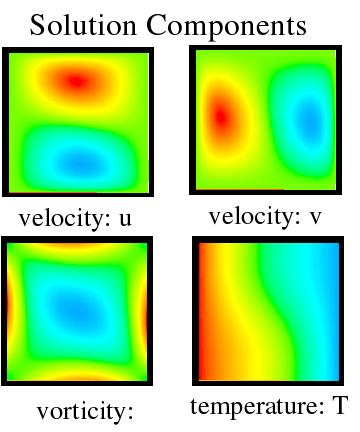
\includegraphics[width=.4\textwidth]{figures/SNES/DrivenCavitySolution}
\vbox{
\begin{itemize}
  \item Velocity-vorticity formulation
  \item Flow driven by lid and/or bouyancy
  \item Logically regular grid
  \begin{itemize}
    \item Parallelized with {\kb DMDA}
  \end{itemize}
  \item Finite difference discretization
  \item Authored by David Keyes
\end{itemize}
}
}
\code{src/snes/examples/tutorials/ex50.c}
\end{frame}

\begin{frame}[fragile]{SNES Example}
\framesubtitle{Driven Cavity Application Context}
\begin{minted}{c}
/* Collocated at each node */
typedef struct {
  PetscScalar u,v,omega,temp;
} Field;

typedef struct {
       /* physical parameters */
   PassiveReal lidvelocity,prandtl,grashof;
       /* color plots of the solution */
   PetscTruth  draw_contours;
} AppCtx;
\end{minted}
\end{frame}

\begin{frame}[fragile]{SNES Example}
\begin{minted}[fontsize=\footnotesize]{c}
DrivenCavityFunction(SNES snes, Vec X, Vec F, void *ptr) {
  AppCtx        *user = (AppCtx *) ptr;
  /* local starting and ending grid points */
  PetscInt       istart, iend, jstart, jend;
  PetscScalar    *f;             /* local vector data */
  PetscReal      grashof = user->grashof;  
  PetscReal      prandtl = user->prandtl;
  PetscErrorCode ierr;

  /* Code to communicate nonlocal ghost point data */
  VecGetArray(F, &f);

  /* Loop over local part and assemble into f[idxloc] */
  /* .... */

  VecRestoreArray(F, &f);
  return 0;
}
\end{minted}
\end{frame}

\begin{frame}[fragile]{SNES Example with local evaluation}
\begin{minted}[fontsize=\footnotesize]{c}
PetscErrorCode DrivenCavityFuncLocal(DMDALocalInfo *info,
                    Field **x,Field **f,void *ctx) {
  /* Handle boundaries ... */
  /* Compute over the interior points */
  for(j = info->ys; j < info->ys+info->ym; j++) {
    for(i = info->xs; i < info->xs+info->xm; i++) {
      /* convective coefficients for upwinding ... */
      /* U velocity */
      u          = x[j][i].u;
      uxx        = (2.0*u - x[j][i-1].u - x[j][i+1].u)*hydhx;
      uyy        = (2.0*u - x[j-1][i].u - x[j+1][i].u)*hxdhy;
      f[j][i].u  = uxx + uyy - .5*(x[j+1][i].omega-x[j-1][i].omega)*hx;
      /* V velocity, Omega ... */
      /* Temperature */
      u             = x[j][i].temp;
      uxx           = (2.0*u - x[j][i-1].temp - x[j][i+1].temp)*hydhx;
      uyy           = (2.0*u - x[j-1][i].temp - x[j+1][i].temp)*hxdhy;
      f[j][i].temp =  uxx + uyy + prandtl
        * (  (vxp*(u - x[j][i-1].temp) + vxm*(x[j][i+1].temp - u)) * hy
           + (vyp*(u - x[j-1][i].temp) + vym*(x[j+1][i].temp - u)) * hx);

}}}
\end{minted}

\begin{center}\small
\$PETSC\_DIR/src/snes/examples/tutorials/ex50.c
\end{center}
\end{frame}
